\section{Wellen / Akustik \kuchling{229} \stoecker{265}}
\subsection{Definitionen räumlicher Elemtarwellen}
\begin{tabular}[]{|p{9cm}|p{9cm}|}
	\hline
	\begin{minipage}{9cm}
		\textbf{Wellengleichung:}\\
			$\ddot{\xi} = u^2 \cdot \xi''(x)$
	\end{minipage} &
	\begin{minipage}[]{9cm}
			$\ddot{\xi}$ = Zweite Ableitung nach der Zeit\\
			$\xi''$ = Zweite Ableitung nach dem Ort
	\end{minipage}\\
	\begin{minipage}[]{9cm}
    	\textbf{Ebene harmonische Welle:}\\
 		$\xi(\vec{r},t)=\xi_0 \sin(\omega t -k\vec{r}+\varphi)$\\ \\		   	
 		$\xi(\vec{r},t)=\xi_0 e^{-j(\omega t-k\vec{r})}$\\ \\ 
 		\textbf{Harmonische Kugelwelle:}\\
 		$\xi(\vec{r},t)=\dfrac{\xi_0}{|\vec{r}|} \sin(\omega
 		t-k|\vec{r}|+\varphi)$\\\\
 		$\xi(\vec{r},t)=\dfrac{\xi_0}{|\vec{r}|} e^{-j(\omega t-k|\vec{r}|)}$\\ 		
    \end{minipage} &
	\begin{minipage}[]{9cm}
    	\vspace{0.2cm}    
    	$\xi({\vec{r},t})$ = Auslenkung am Ort $\vec{r}$ zur Zeit $t$\\
		$\xi_0$ = Amplitude $[1]$\\
		$k$ = Wellenzahl $[\frac{1}{m}]$\\
		$\vec{r}$ = Ortsvektor $[m]$\\
		$\omega$ = Kreisfrequenz $[\frac{1}{s}]$\\
		$\varphi$ = Phasenverschiebung $[rad]$\\    
		$\lambda$ = Wellenlänge $[m]$\\
		$u$ = Wellengeschwindigkeit $[\frac{m}{s}]$\\
		$f$ = Frequenz $[Hz]$\\
		$T$ = Periodendauer $[s]$\\
    \end{minipage} \\
	\hline
\end{tabular}

\subsection{Wichtige Beziehungen}
$\boxed{k=\dfrac{\omega}{u}=\dfrac{2\pi}{\lambda}}$\quad
$\boxed{u=\dfrac{\omega}{k} = \lambda \cdot f}$ \quad
$\boxed{\lambda=\dfrac{2\pi}{k}=\dfrac{u}{f}}$ \quad
$\boxed{\omega=2\pi f=\dfrac{2\pi}{T}}$ \quad
$\boxed{f=\dfrac{\omega}{2\pi}=\dfrac{u}{\lambda}=\dfrac{1}{T}}$ \quad
$\boxed{T=\dfrac{1}{f}=\dfrac{2\pi}{\omega}}$ \quad
$\boxed{\varphi=\omega t-k|\vec{r}|}$

\subsection{Wellengeschwindigkeit \kuchling{233} \stoecker{267}}
\renewcommand{\arraystretch}{1.5}
\begin{tabular}{| p{6cm} | p{6cm} | p{6cm} |}
\hline
\textbf{Elastisch}e L"angs-/ Longitudinalwelle & \textbf{Elastisch}e Quer-/ Transversalwelle & Transversalwellen bei \textbf{Saite} oder Seil\\
$u=\sqrt{\dfrac{E}{\varrho}}$ & $u=\sqrt{\dfrac{G}{\varrho} }\quad$ mit $G=\dfrac{E}{2(1+\mu)}$ &
$u=\sqrt{\dfrac{F}{\varrho\,A}}=\sqrt{\dfrac{F}{\varrho}+\dfrac{\pi\,E\,A}{\varrho\,\lambda^2}}$
\\ $E$: Elastizit"atsmodul, $\rho$ = Dichte& $G$: Schubmodul, $\mu$ = Poisson-Zahl & $F$: Spannkraft, $E$:
Elastizit"atsmodul \\
\hline

Schwerewellen in \textbf{tiefem Wasser} & Schwerewellen in \textbf{flachem Wasser}& \textbf{Kapillarwellen}\\
$u=\sqrt{\dfrac{g\,\lambda}{2\pi}}$&$u=\sqrt{g\,h}$&$u=\sqrt{\dfrac{2\pi\,\sigma}{\varrho\,\lambda}}$\\
($\lambda \ll h$) & ($\lambda \gg h$)  & $\sigma$: Oberfl"achenspannung \\
\hline

Schallwellen in \textbf{Fluide}n & Schallwellen in \textbf{Gas}en & \textbf{Elektromagnetische} Wellen\\
$u=\sqrt{\dfrac{1}{\varrho\,\kappa}}$&$u=\sqrt{\dfrac{\varkappa\,p}{\varrho}}=\sqrt{\dfrac{\varkappa\,R\,T}{M}}$&
$u = \dfrac{c}{n}$\\
$\kappa$: Kompressibilit"at &$p$: Druck, $M$: Molmasse& n= Brechungsindex\\
& $\varkappa$: Adiabatenexponent&\\
\hline
\multicolumn{3}{|l|}{
	$M_{Luft}=
	0.02883 \dfrac{kg}{mol} = 28.83 \dfrac{g}{mol} \hspace{1.5cm}
	R=8.3145 \dfrac{J}{mol\cdot K} \hspace{1.5cm}
	\varkappa_{Luft}=1.4 \hspace{1.5cm}
	\text{T: }C^\circ+273,15K$
}\\
\hline
\end{tabular}
\renewcommand{\arraystretch}{1}

%\subsection{Stehende Welle}

%\begin{tabular}{|ll|lll|}
%	\hline
%	Laufzeit
%		& $ t = \dfrac{2\cdot l}{u} \qquad$
%		& \textbf{Intereferenzbedinung}
%		& $T_n = \dfrac{t}{n} = \dfrac{1}{n} \cdot \dfrac{2\cdot l}{u} \qquad$ 
%		& \parbox{6cm}{
%			$l$ = Länge des Objekts\\
%			$n$ = \textbf{ganzes} Vielfaches}\\
%	\hline
%\end{tabular}

\subsection{Eigenschwingungen Allg. /Akustik \kuchling{334} \stoecker{294}}
\renewcommand{\arraystretch}{2.5}
\begin{tabular}{|l|llll|}
\hline
\textbf{Allgemein}
	& Eigenfrequenz: 
	& $ f_n=\dfrac{1}{T_n} = n\cdot \dfrac{u}{2 \cdot l}$
	& Wellenlänge:
	& $\lambda_n=\dfrac{u}{f_n}=\dfrac{2\cdot l}{n}$\\
\hline
\textbf{Saiten}
	& Grundfrequenz: 
	& $ f_n= n \cdot \dfrac{1}{2l}\sqrt{\dfrac{F}{\varrho\,A}} = n \cdot \dfrac{1}{2l}\sqrt{\dfrac{\sigma}{\varrho}} $
	& 
	& $\lambda_n=\dfrac{2l}{n}$ \quad ($n=1,2,3,...$)\\
\hline
\textbf{Pfeifen} & Offen:
 	& $f_n=n\cdot \dfrac{1}{2l}\,u_{\text{Gas}}=n\cdot \dfrac{1}{2l}\sqrt{\dfrac{\varkappa\,R\,T}{M}}$ 
	& 
	& $\lambda_n=\dfrac{2l}{n}$ \quad ($n=1,2,3,...$)\\
& Gedeckt: 
 	& $ f_{(2n-1)}=\dfrac{2n-1}{4l}\sqrt{\dfrac{\varkappa\,R\,T}{M}}$
	& 
	& $\lambda_n=\dfrac{4l}{2n-1}$ \quad ($(2n-1)=1,3,5,...$) \\ 
\hline
\textbf{Membranen}
 	& &
 	$f_{mn}=\dfrac{1}{2}\sqrt{\dfrac{F}{\mu}}\sqrt{\dfrac{m^2}{a^2}+\dfrac{n^2}{b}}$ 
	& \multicolumn{2}{l|}{\parbox{8cm}{$m,n$: Anz. Oberwellen und $a,b$:
	L"ange/Breite \\
	$\mu$: Masse / Fläche; $F$: Spannkraft / Länge}} \\ \hline
\end{tabular}

\subsection{Doppler-Effekt \kuchling{342} \stoecker{277}}
\begin{tabular}{|l|l|l|}
\hline
\begin{minipage}[]{4cm}
		\small
		\vspace{.2cm}
		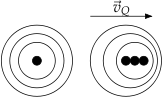
\includegraphics[width=3cm]{./bilder/doppler.png}\\
		Ruhende \& bewegte Punktquelle \\ \\ \\
		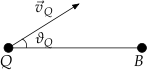
\includegraphics[width=3cm]{./bilder/doppler-bewegte-quelle.png}\\
		Bewegte Punktquelle \\ \\ \\
		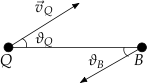
\includegraphics[width=3cm]{./bilder/doppler-beide-bewegt.png} \\
		Bewegter Beobachter \& bewegte Quelle \\
		\end{minipage}
	& \begin{minipage}[]{7cm}
      	\renewcommand{\arraystretch}{2}
      	\vspace{.2cm}
	  	\textbf{Bewegte Quelle, ruhender Beobachter} \\
	  	$f_B = \dfrac{1}{1 \mp  \dfrac{v_Q}{u}} f_Q$ \qquad \parbox{3cm}{- auf Hörer zu \\
	  				 + von Hörer weg}\\
	  	$f_B = \dfrac{1}{1 - \dfrac{v_Q}{u} \cos(\vartheta_Q)} f_Q$ \\
	  	\vspace{.5cm}\\
	  	\textbf{Ruhende Quelle, bewegter Beobachter} \\
	  	$f_B = \left(1 \pm \dfrac{v_B}{u}\right) f_Q$ \qquad + auf Quelle zu \\
	  	$f_B = \left(1 + \dfrac{v_B}{u} \cos(\vartheta_B)\right) f_Q$ \\
	  	\vspace{.5cm}\\
	  	\textbf{Allgemein} \\
	  	$f_B = \dfrac{u + v_B \cos(\vartheta_B)}{u - v_Q \cos(\vartheta_Q)} f_Q$ \\
	  	\vspace{.5cm}\\
	  	\textbf{Optischer (transversaler) Dop.-Effekt } \\
	  	$f_B = \dfrac{\sqrt{1 - \beta^2}}{1 - \beta \cos \vartheta_{rel}} f_Q \qquad \beta =
	  	\dfrac{v_{rel}}{c}$ \\ 
	  	$ \vec{v}_{rel} = \vec{v}_B - \vec{v}_Q \vspace{.5cm}\\
	  	\textbf{Schwebungsfrequenz}\\
	  	\Delta f = |f_{Empfangen} - f_{Gesendet}|$ \vspace{.2cm}
      	\renewcommand{\arraystretch}{1}
    	\end{minipage}
	& \parbox{6.5cm}{
		$f_B \;$ gehörte Frequenz \\
		$f_Q \;$ gesendete Frequenz \\
		$v_B \;$ Geschwindigkeit Beobachter \\
		$v_Q \;$ Geschwindigkeit Quelle\\
		$u \;$ Schallgeschwindigkeit\\
		$v_{rel} \;$ Relativgeschwindigkeit zw. Q und B\\
		$\vartheta_{rel} \;$ Winkel zwischen $\vec{v}_{rel}$ und $\overline{BQ}$
		} \\
\hline
\end{tabular}

\begin{minipage}{10cm}
	\subsection{Machscher Kegel \kuchling{344} \stoecker{278}}
	\begin{tabular}{ll}
	\parbox{5cm}{
		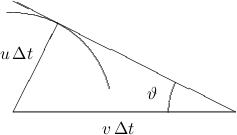
\includegraphics[width=4cm]{./bilder/machscher-kegel.png}}
		& 
		\parbox{5cm}{$\sin(\vartheta)=\dfrac{u}{v} = \dfrac{1}{M}$ \\ \\
		Machzahl: $M=\dfrac{v}{u}$}
	\end{tabular}
\end{minipage}
\begin{minipage}{8cm}
	\subsection{Lichtwellen}
		Lichtgeschwindigkeit: $ c = \dfrac{1}{\sqrt{\mu_0 \cdot \epsilon_0}} \qquad \qquad$ \\
		Intensität: $I = \dfrac{1}{2} \cdot \sqrt{\dfrac{\epsilon_0}{\mu_0}} \cdot {E_0}^2 \quad$ in $[W/m^2]$
\end{minipage}


\subsection{Optische Länge}
Durchqueren Wellen Medien, muss mit optischen Längen gerechnet werden.\qquad 
$s$ wird zu $n\,s$ \qquad $\lambda$ wird zu $\dfrac{\lambda}{n}$



\subsection{"Uberlagerung / Interferenz \kuchling{233, 235} \stoecker{272, 354}}
\setlength{\tabcolsep}{5pt}
\renewcommand{\arraystretch}{2}
\subsubsection{Interferenzbedingungen}
\begin{tabular}{p{11cm} p{7cm}}
\begin{minipage}[]{11cm}
	\begin{tabular}{|l|l|l|}
	\hline
	& \textbf{Phase} & \textbf{Weg} \\
	\hline
	Konstruktiv: 
		& $k_0(n\cdot \Delta x)=m \, 2\pi$
		& $n \, \Delta x = m \, \lambda$ \\
	Destruktiv: 
	 	& $k_0(n\cdot \Delta x)=(2m+1)\pi$
	 	& $n \, \Delta x = (2m+1) \frac{\lambda}{2}$ \\
	\hline
	\end{tabular}\\
	\end{minipage}
	& \parbox{8cm}{$k_0 = \dfrac{2\pi}{\lambda_0}$ = Wellenzahl im Vakuum\\
	$ \lambda_0$ = Wellenlänge im Vakuum\\
	n = Brechungsindex, Kuchling Tab 39, S.653\\
	$n\cdot \Delta x$ = optische Gangdifferenz}
\end{tabular}\\
\textbf{Phasensprung:}
		\parbox{16cm}{Ein Phasensprung um $\pi$ bzw. $\frac{\lambda}{2}$ findet bei
		\textbf{Reflektion} an einem härteren oder optisch dichterem Material
		(\textbf{höheres $n$}) statt.}
		
\subsection{Remission/Transmission}
\textbf{Remission} $R= \left(\dfrac{f-1}{f+2}\right)^2$ mit $ f = \dfrac{n_1}{n_2}$\hspace{2cm} \textbf{Transmission} $T = 1-R$  

\subsection{Schallmessung \kuchling{348} \stoecker{287}}
\setlength{\tabcolsep}{5pt}
\renewcommand{\arraystretch}{2.4}
\begin{tabular}{>{\bfseries}ll}
Welle: & $\xi=\xi_0\sin(\omega t-kx)$ \qquad $\xi_0$ Schallausschlag \qquad
$[\xi]$: m
\\
Schallschnelle: & $v=v_0\cos(\omega t-kx)\qquad\rightarrow\qquad v=\dot{\xi}=\omega\xi_0\cos(\omega t-kx)\rightarrow \dfrac{v_0}{\omega}=\xi_0$\\
Schall(wechsel)druck: & $\tilde p=\Delta p_0 \cos(\omega t-kx)$ \\
Druckamplitude: & $\Delta p_0=Z\cdot v_0$ \qquad Schallimpedanz $Z=\varrho
\cdot u$\\ 
Effektivwert: & $p_{\text{eff}} = \dfrac{\Delta p_0}{\sqrt{2}}$\\
Schallintensität: & $I=\dfrac{1}{2}\,\varrho\, v_0^{\,2}\,u =
\dfrac{1}{2}\varrho\,\omega^2\, \xi_0^{\,2}\,u =  \dfrac{\Delta
p_0^{\,2}}{2\cdot Z}$ \qquad $\xi_0$ Schallausschlag; $\varrho$ Dichte des Mediums\\  

Schallpegel [dB] : & $\boxed{L_I=10\cdot \log\left(\dfrac{I}{I_0}\right)}$\qquad
$I_0=10^{-12}$ W/m$^2$ \qquad $L_I=L_p$ f"ur Z=400kg/m$^2$s @ 20$^{\circ}$C\\
Schalldruckpegel: & $L_p=20\cdot\log\left(\dfrac{p_{\text{eff}}}{p_{\text{eff}_0}}\right)= 20\cdot\log\left(\dfrac{\Delta p_0}{\sqrt{2}\cdot p_{\text{eff}_0}}\right)$\qquad $p_{\text{eff}_0}=2\cdot 10^{-5}$ Pa\\
Schallschnellenpegel: & $L_v=20\cdot\log\left(\dfrac{v_{\text{eff}}}{v_{\text{eff}_0}}\right)$ \qquad $v_{\text{eff}_0}=5\cdot10^{-8}$m/s \\
Schallleistungspegel: & 
$L_P = 10\cdot\log\left(\dfrac{P}{P_0}\right)$ \qquad  $P_0=10^{-12}$W\\
Schallfluss: & $\vec q=\int\limits_{A}{\vec v\cdot dA}$\\
Wellengeschwindigkeit: & $u=\sqrt{\dfrac{1}{\varrho\,\kappa}}=\underbrace{\sqrt{\dfrac{\varkappa\,p}{\varrho}}=\sqrt{\dfrac{\varkappa\,R\,T}{M}}}_{\text{f"ur Gase}}$ \qquad (Schallgeschwindigkeit) $\kappa$: Kompressibilit"at \quad\\
& $\Rightarrow\dfrac{\Delta V}{V}=-\kappa\cdot\Delta p$ \qquad ($p\cdot V=\text{const}\,\,@\,\,T_{\text{const}}$ bzw. $p\cdot V^{\varkappa}=\text{const}$) \\
Lautstärke: & $S=2^{0.1\cdot(L_S-40)}$ \qquad $L_S=$ Lautst"arkepegel [phon] = $L_P$ @ 1kHz, H"orschwelle 4phon\\
Ebene Welle & (z.B. Parabolspiegel) $\rightarrow$ konstantes I, keine geom. D"ampfung nur Luftd"ampfung\\
& $\boxed{L_2=L_1-K\cdot(r_2-r_1)}$ f"ur $d<<r\quad\rightarrow\quad$ $I_2=\dfrac{P}{4\pi(r+d)^2}\approx\dfrac{P}{4\pi r^2}=I_1$\quad$I=$konstant\\
\parbox{3cm}{Kugelwellen\\
(Punktquellen)}: &  $I=\dfrac{P}{4\pi r^2}\quad\rightarrow\quad \sim\dfrac{1}{r^2}$ und $\dfrac{I_2}{I_1}=\dfrac{r_1^{\,2}}{r_2^{\,2}}$  \\
&$\boxed
{L_2=L_1-\underbrace{20\cdot\log\left(\dfrac{r_2}{r_1}\right)}_{\text{geom. D"ampfung}}-\underbrace{K\cdot(r_2-r_1)}_{\text{Luftd"ampfung}}}$\quad mit $K$: Schalldämpfung [dB/m]\\
\parbox{3cm}{Zylinderwellen\\
(Linienquellen)}: &$I=\dfrac{P}{l\,2\pi r}\quad\rightarrow\quad \sim\dfrac{1}{r} \quad \Rightarrow \boxed{L_2=L_1-10\cdot\log\left(\dfrac{r_2}{r_1}\right)-K\cdot(r_2-r_1)}$ \\
Schalld"ammung: & $\boxed{R=10\,\log\left(\dfrac{P_1}{P_2}\right)}$ \\
Phasensprung & um $\lambda/2$, $\pi$ bei Reflexion w"ahrend "Ubergang von gasf"ormig $\rightarrow$ fest  \\
Infra-/Ultraschall & Infraschall $<$ 16Hz...20kHz $<$ Ultraschall ...10GHz $<$ Hyperschall\\
\end{tabular}
\renewcommand{\arraystretch}{\arraystretchOriginal}

\subsection{Wellenoptik}

\subsubsection{Prinzip von Huygens \kuchling{229}}
Jeder Punkt einer Welle ist Zentrum einer neuen Kugelwelle  
(sogenannte Huygens‘sche Elementarwelle). 
Die Wellenfront zu einem späteren Zeitpunkt ist die Einhüllende dieser Huygens'schen Elementarwellen.\\

\begin{minipage}{9.5cm}
	\subsubsection{Beugung am Doppelspalt}
	\begin{minipage}{4.5cm}
	\textbf{Minimum n-ter Ordnung}\\
		$\sin(\varphi_n) \cdot s = (2n + 1)\cdot \frac{\lambda}{2} $\\
	\textbf{Maximum n-ter Ordnung}\\
			$\sin(\varphi_n) \cdot s = n \cdot \lambda $\\ 
			\\
		\begin{minipage}{4.5cm}
			$\lambda$ = Wellenlänge des Lichts\\
			$s$ = Spalt-Abstand\\
			$\varphi_n$ = Winkel n-ter Ordnung\\
			$n$ = 0,1,2,... = Ordnung
		\end{minipage}
	\end{minipage}
	\begin{minipage}{4cm}
		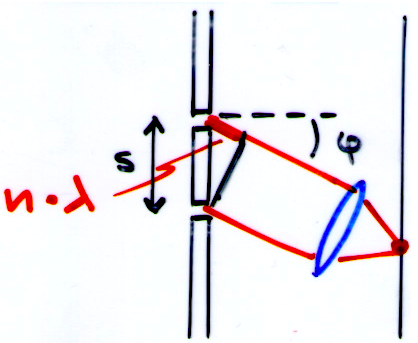
\includegraphics[width = 4cm]{./bilder/beugung-doppelspalt}
	\end{minipage}
\end{minipage}
\begin{minipage}{9cm}
	\subsubsection{Beugung am Einfachspalt}
	\begin{minipage}{4.5cm}
	\textbf{Minimum n-ter Ordnung}\\
		$\sin(\varphi_n) \cdot s = n \cdot \lambda $\\ 	
	\textbf{Maximum n-ter Ordnung}\\
		$\sin(\varphi_n) \cdot s = (2n + 1)\cdot \frac{\lambda}{2} $\\	
		\\
		\begin{minipage}{4.5cm}
			$\lambda$ = Wellenlänge des Lichts\\
			$s$ = Spalt-Abstand\\
			$\varphi_n$ = Winkel n-ter Ordnung\\
			$n$ = 0,1,2,... = Ordnung
		\end{minipage}
	\end{minipage}
	\begin{minipage}{4cm}
		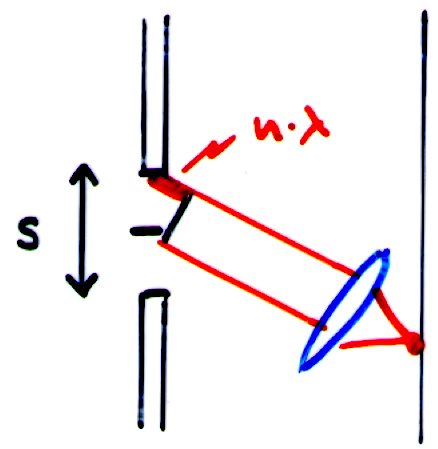
\includegraphics[width = 4cm]{./bilder/beugung-einfachspalt}
	\end{minipage}
\end{minipage}


\subsubsection{Beugung am Gitter}
\begin{minipage}{6cm}
	\textbf{Hauptmaximum n-ter Ordnung}\\
	$\boxed{\sin(\varphi_n) \cdot d = n \cdot \lambda}$\\
	\\
	\begin{minipage}{6cm}
		$\lambda$ = betrachtete Lichtwellenlänge\\
		$d$ = konstanter Spaltenabstand\\
		$\varphi_n$ = Maximumwinkel n-ter Ordnung \\
		$n$ = 0,1,2,... = Ordnung
	\end{minipage}
\end{minipage}
\begin{minipage}{5cm}
	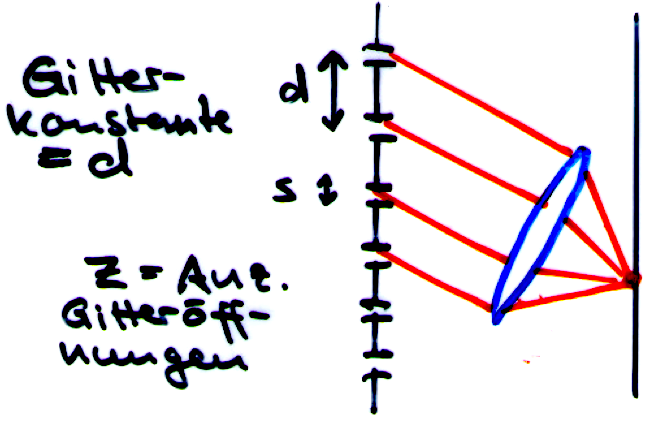
\includegraphics[width = 4cm]{./bilder/beugung-gitter}
\end{minipage}
\begin{minipage}{8cm}
	\textbf{Bedingungen für optimales optisches Gitter}
	\begin{enumerate}
		\item Möglichst kleine Gitterkonstante $\mathbf{d}$
		\item Möglichst grosse Gitter-Zahl $\mathbf{z}$
		\item Möglichst kleine Gitter-Breite $\mathbf{s}$
	\end{enumerate}
\end{minipage}\\
\\ \\
\begin{minipage}{18cm}
	\begin{tabular}{lllll}
	\parbox{4.5cm}{Intentitäts-Verteilung	\textbf{Gitter}}
		& $\approx$
		& \parbox{5.5cm}{Formfaktor\\
				{\small = Intensitätsverteilung \textbf{Einzelspalt}}}
		& $\times$
		& \parbox{6cm}{Interferenzfunktion\\
						{\small = Intensitätsverteilung \textbf{Doppelspalt}}}\\	
	\parbox{4.5cm}{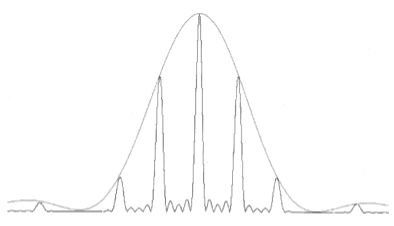
\includegraphics[width = 4.5cm]{./bilder/intensitaetsverteilung-gitter}}	
		& $\approx$
		& \parbox{4.5cm}{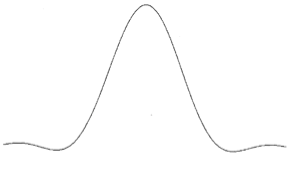
\includegraphics[width = 4.5cm]{./bilder/intensitaetsverteilung-einzelspalt}}
		& $\times$
		& \parbox{4.5cm}{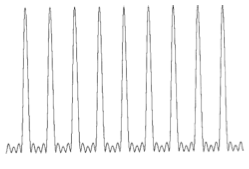
\includegraphics[width = 4.5cm]{./bilder/intensitaetsverteilung-doppelspalt}}
		\\			
	\end{tabular}
	Dabei entsteht immer z-2 Neben-Maxima.
\end{minipage}

\subsubsection{Babinet-Theorem}
Komplemetäre Strukturen (also Negativ und Positiv) liefern gleiche Beugungsbilder

\newpage
